\section{Introduction}
do we need this?

\section{Implementation}
do we need this?

\section{Analysis of the performance}

\paragraph{Learning curve}

\begin{figure}[h!]
\centering
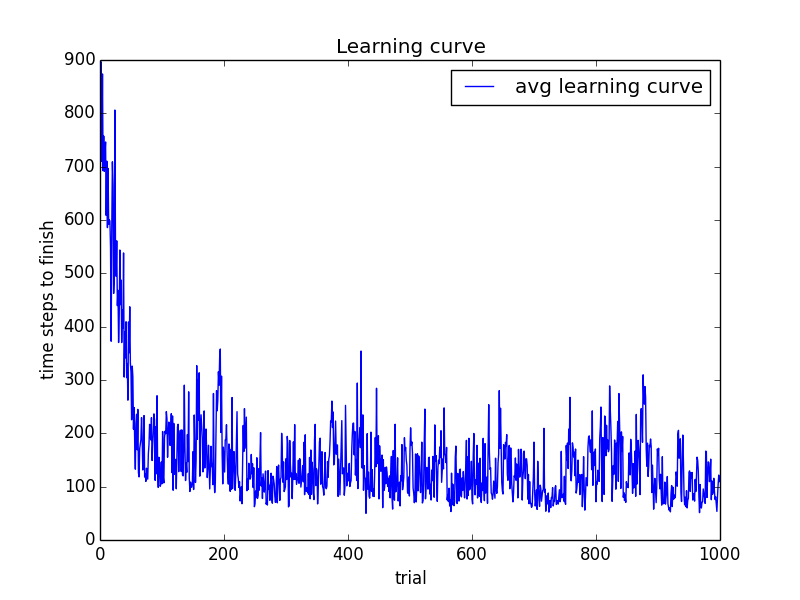
\includegraphics[width=0.8\textwidth]{figures/learning_curve.png}
\label{fig:lcurve}
\caption{Learning curve, averaged over $10$ independent learning agents}
\end{figure}

The learning curve of implemented algorithm can be seen in the
Figure~\ref{fig:lcurve}. It is an average over $10$ independent learning runs in
order to reduce the high oscillations of a single run. The curve initially
decreases, what means that in every next trial the agent takes less time to
finish the track. In other words, it indeed does learn the topology of the track
and the location of the reward. The learning curve reaches the plateau after
approximately $100$ trials and after that the learning stops decreasing and
oscillates instead, between the values of $100$ and $300$ timesteps to finish
the track. The meaning of that is that the agent has learnt enough information
about the environment and starts to exploit it extensively. The exploration that
happens is not enough to find the better solutions.

\paragraph{Integrated reward}

\begin{figure}[h!]
\centering
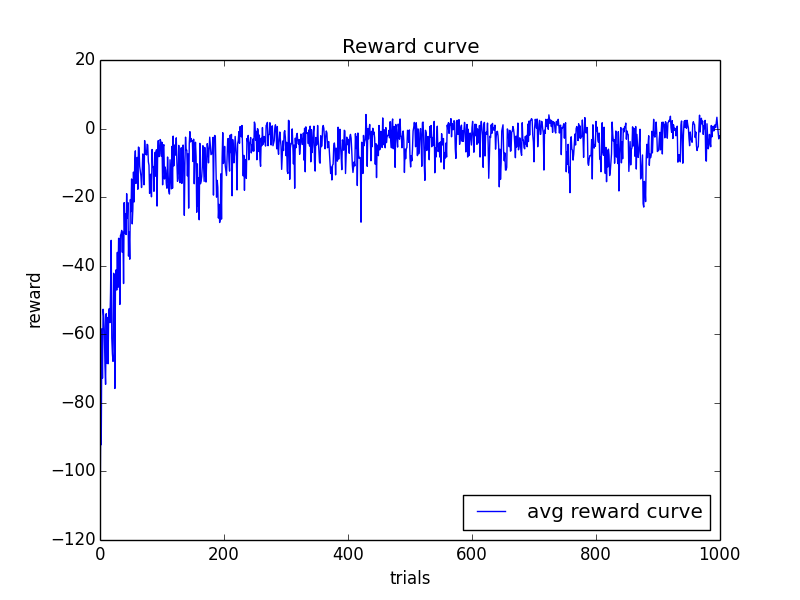
\includegraphics[width=0.8\textwidth]{figures/reward_curve.png}
\label{fig:rcurve}
\caption{Reward curve, averaged over 10 independent learning cars}
\end{figure}

The reward curve is plotted in the Figure~\ref{fig:rcurve}. It highly resembles
the learning curve, despite being negative and scaled. The consistency between
the two curves confirms the correlation between the obtained reward and the
learning.

\paragraph{Exploration-exploitation}

\paragraph{Navigation map}


\section{Car race}
comment on our changes (if we actually do this)
